\documentclass[14pt, a4paper]{extarticle}
\usepackage{GOST}
\usepackage{array}
\usepackage{verbatim}
\usepackage[detect-all]{siunitx}
\usepackage{amsmath}
\usepackage{amssymb}
\usepackage[utf8]{inputenc}
\usepackage{hyperref}

\usepackage{ifthen}


\usepackage{tempora}



\makeatletter
\renewcommand\@biblabel[1]{#1.}
\makeatother

% Для листинга кода:
\usepackage{listings}
\lstset{ %
	language=c++,                 % выбор языка для подсветки (здесь это С)
	basicstyle=\small\sffamily, % размер и начертание шрифта для подсветки кода
	numbers=left,               % где поставить нумерацию строк (слева\справа)
	numberstyle=\tiny,           % размер шрифта для номеров строк
	stepnumber=1,                   % размер шага между двумя номерами строк
	numbersep=5pt,                % как далеко отстоят номера строк от подсвечиваемого кода
	showspaces=false,            % показывать или нет пробелы специальными отступами
	showstringspaces=false,      % показывать или нет пробелы в строках
	showtabs=false,             % показывать или нет табуляцию в строках
	frame=single,              % рисовать рамку вокруг кода
	tabsize=2,                 % размер табуляции по умолчанию равен 2 пробелам
	captionpos=t,              % позиция заголовка вверху [t] или внизу [b] 
	breaklines=true,           % автоматически переносить строки (да\нет)
	breakatwhitespace=false, % переносить строки только если есть пробел
	escapeinside={\#*}{*)}   % если нужно добавить комментарии в коде
}


%для графиков
\usepackage{pgfplots}
\usepackage{filecontents}
\usetikzlibrary{datavisualization}
\usetikzlibrary{datavisualization.formats.functions}

\begin{document}
	
	\begin{table}[ht]
		\centering
		\begin{tabular}{|c|p{400pt}|} 
			\hline
			\begin{tabular}[c]{@{}c@{}} 
\includegraphics[scale=1]{baum.jpg} \\\end{tabular} &
			\footnotesize\begin{tabular}[c]{@{}c@{}}\textbf{Министерство~науки~и~высшего~образования~Российской~Федерации}\\\textbf{Федеральное~государственное~бюджетное~образовательное~учреждение}\\\textbf{~высшего~образования}\\\textbf{«Московский~государственный~технический~университет}\\\textbf{имени~Н.Э.~Баумана}\\\textbf{(национальный~исследовательский~университет)»}\\\textbf{(МГТУ~им.~Н.Э.~Баумана)}\\\end{tabular}  \\
			\hline
		\end{tabular}
	\end{table}
	\noindent\rule{\textwidth}{4pt}
	\noindent\rule[14pt]{\textwidth}{1pt}
	\hfill 
	\noindent
	\makebox{ФАКУЛЬТЕТ~}%
	\makebox[\textwidth][l]{\underline{~«Информатика и системы управления»~~~~~~~~~~~~~~~~~~~~~~~~~~~~~~~~~}}%
	\\
	\noindent
	\makebox{КАФЕДРА~}%
	\makebox[\textwidth][l]{\underline{~«Программное обеспечение ЭВМ и информационные технологии»~}}%
	\\
	
	\begin{center}
		\vspace{1.5cm}
		{\bf\huge Отчёт\par}
		{\bf\Large по лабораторной работе № 1 (часть 2)\par}
		\vspace{0.7cm}
	\end{center}
	
	
	\noindent
	\makebox{\large{\bf Название:}~~~}
	\makebox[\textwidth][l]{~~~\large\underline{~Функции системного таймера  и пересчет~}}\\
	\indent\indent\makebox[\textwidth][l]{\large\underline{~~~~~~~~~~~~~~~~~~~~~~динамических приоритетов.~~~~~~~~~~}}
	
	\noindent
	\makebox{\large{\bf Дисциплина:}~~~}
	\makebox[\textwidth][l]{\large\underline{~Операционные системы~~~~~~~~~~~~~~~~~~~~~~~~~~}}\\
	
	\vspace{1.5cm}
	\noindent
	\begin{tabular}{l c c c c c}
		Студент      & ~ИУ7-55Б~               & \hspace{2.5cm} & \hspace{2cm}                 & &  Д.В. 
		Сусликов \\\cline{2-2}\cline{4-4} \cline{6-6} 
		\hspace{3cm} & {\footnotesize(Группа)} &                & {\footnotesize(Подпись, дата)} & & {\footnotesize(И.О. Фамилия)}
	\end{tabular}
	
	\noindent
	\begin{tabular}{l c c c c}
		Преподаватель & \hspace{5cm}   & \hspace{2cm}                 & & ~~~~~~Н.Ю. Рязанова~~~~~~\\\cline{3-3} \cline{5-5} 
		\hspace{3cm}  &                & {\footnotesize(Подпись, дата)} & & {\footnotesize(И.О. Фамилия)}
	\end{tabular}
	
	\vspace{0.6cm}
	\begin{center}	
		\vfill
		\large \textit {Москва, 2020}
	\end{center}
	
	\thispagestyle {empty}
	\pagebreak
	
	% СОДЕРЖАНИЕ 
	\clearpage
	\tableofcontents
	
	
	% ВВЕДЕНИЕ
	\clearpage
	\section{Функции системных таймеров в защищенном режиме}
	\subsection{Windows}
	\textbf{По тику:}
	\begin{itemize}
		\item[1)] Обновление системного времени (инкремент счетчика системного времени); 
		\item[2)] Декремент показания счетчика, отслеживающего продолжительность
		работы текущего потока (декремент кванта потока); 
		\item[3)] Декремент показаний счетчиков отложенных задач.
	\end{itemize}
	
	\textbf{По главному тику:}
	\begin{itemize}
			\item[1)] Инициализация диспетчера настройки баланса (освобождение объекта "событие" каждую секунду).
	\end{itemize}
	
	\textbf{По кванту:}
	\begin{itemize}
		\item[1)] Инициализация диспетчеризации потоков (добавление соответствующего
		объекта DPC в очередь). 
	\end{itemize}

	\subsection{Unix/Linux}
	\textbf{По тику:}
	\begin{itemize}
		\item[1)] Обновление статистики использования процессора текущим процессом (инкремент счетчика времени использования процессора текущим процессом); 
		\item[2)] Обновление часов и других таймеров системы (инкремент часов и других таймеров системы); 
		\item[3)] Проверка необходимости выполнения отложенного вызова, при нахождении ожидающего вызова
		выставляется флаг, указывающий на необходимость запуска обработчика отложенного вызова.
	\end{itemize}
	
	\clearpage
	\textbf{По главному тику:}
	\begin{itemize}
		\item[1)] Добавление функций планировщика, например пересчет приоритетов, в очередь отложенных вызовов;
		\item[2)] Пробуждение системных процессов, таких как swapper и pagedaemon
		(процедура wakeup перемещает дескрипторы процессов из очереди "спящих" в очередь "готовых к выполнению");
		\item[3)] Декремент счетчиков времени, оставшегося до отправления сигналов тревоги:
			\subitem3.1) SIGALARM - сигнал будильника реального времени.
			\subitem3.2) SIGPROF - сигнал будильника профиля.
			\subitem3.3) SIGVTALARM - сигнал будильника виртуального времени.
	\end{itemize}
	
	\textbf{По кванту:}
	\begin{itemize}
		\item[1)] Посылка текущему процессу сигнала SIGXCPU, если тот превысил
		выделенный ему квант использования процессора (процессорного
		времени).
	\end{itemize}
	 
	\section{Пересчет динамических приоритетов}
	В Windows и Unix/Linux могут пересчитываться только приоритеты пользовательских процессов.
	
	\subsection{В Windows}	
	В Windows реализуется приоритетная, вытесняющая система планирования, при
	которой всегда выполняется хотя бы один работоспособный (готовый) поток с самым высоким приоритетом, с той оговоркой, что конкретные, имеющие высокий
	приоритет и готовые к запуску потоки могут быть ограничены процессами, на которых им разрешено или предпочтительнее всего работать.\par
	
	В то время как у процесса имеется только одно базовое значение приоритета, у каждого потока имеется два значения приоритета: текущее (динамическое) и базовое.
	
	Исходный базовый приоритет потока наследуется от базового приоритета процесса.
	Процесс по умолчанию наследует свой базовый приоритет у того процесса, который
	его создал.
	
	Как правило, пользовательские приложения и службы запускаются с обычным
	базовым приоритетом (normal), поэтому их исходный поток чаще всего
	выполняется с уровнем приоритета 8.
	
	Повысить или понизить приоритет потока в динамическом диапазоне можно в
	любом приложении, но у вас должны быть привилегии, позволяющие повышать
	приоритет, использующийся при планировании для ввода значения в пределах
	динамического диапазона. 
	
	
	Windows использует 32 уровня приоритета, от 0 до 31 (31 —
	наивысший). Эти значения разбиваются на категории следующим образом:
	\begin{itemize}
		\item[1)] шестнадцать уровней реального времени (от 16 до 31);
		\item[2)] шестнадцать изменяющихся уровней (от 0 до 15), из которых уровень 0 зарезервирован для потока обнуления страниц. 
	\end{itemize}

	Уровни приоритета потоков назначаются c двух позиций: от Windows API и от ядра
	Windows. Сначала Windows API распределяет процессы по классу приоритета, который им присваивается
	при создании.
	
	\begin{itemize}
		\item[1)] реального времени — Real-time (4);
		\item[2)] высокий — High (3);
		\item[3)] выше обычного — Above Normal (6);
		\item[4)] обычный — Normal (2);
		\item[5)]ниже обычного — Below Normal (5);
		\item[6)] уровень простоя — Idle (1).		
	\end{itemize}
	 
	 А затем внутри этих процессов назначается приоритет отдельным потокам. Числа в скобках прибавляются к базовому приоритету процесса:
	 
	 \begin{itemize}
	 	\item[1)] критичный по времени — Time-critical (15);
	 	\item[2)] наивысший — Highest (2);
	 	\item[3)] выше обычного — Above-normal (1);
	 	\item[4)] обычный — Normal (0);
	 	\item[5)] ниже обычного — Below-normal (–1);
	 	\item[6)] самый низший — Lowest (–2);
		\item[7)] уровень простоя — Idle (–15).		
	 \end{itemize}
 
	 Таким образом, у каждого потока два приоритета: текущий и базовый. Решения,
	 связанные с планированием, принимаются на основе текущего приоритета.
	 Отображение Windows-приоритета на внутренние номерные приоритеты Windows
	 показано в таблице. 
	 
	 \begin{table}
	 	\begin{center}
	 		\begin{tabular}{|l|p{45pt}|p{45pt}|p{45pt}|p{45pt}|p{45pt}|p{45pt}|}
	 			\hline
	 			{} & Real-time & High & Above-Normal & Normal & Below-Normal & Idle\\
	 			\hline
	 			Time Critical & 31 & 15 & 15 & 15 & 15 & 15 \\
	 			\hline
	 			Highest & 26 & 15 & 12 & 10 & 8 & 6 \\
	 			\hline
	 			Above Normal & 25 & 14 & 11 & 9 & 7 & 5 \\
	 			\hline
	 			Normal & 24 & 13 & 10 & 8 & 6 & 4 \\
	 			\hline
	 			Below Normal & 23 & 12 & 9 & 7 & 5 & 3 \\
	 			\hline
	 			Lowest & 22 & 11 & 8 & 6 & 4 & 2 \\
	 			\hline
	 			Idle & 16 & 1 & 1 & 1 & 1 & 1 \\
	 			\hline
	 		\end{tabular}
	 	\end{center}
	 	\caption*{Соответствие между приоритетами ядра Windows и Windows API}
	 	\label{tbl:priority}
	 \end{table}
	\newpage
	Система динамически повышает приоритет текущего потока в следующих случаях:
	\begin{itemize}
		\item[1)] вследствие событий планировщика или диспетчера;
		\item[2)] вследствие завершения ввода/вывода;
		\item[3)] вследствие ввода из пользовательского интерфейса;
		\item[4)] вследствие слишком продолжительного ожидания ресурса исполняющей системы;
		\item[5)] в случае, когда готовый к запуску поток не был запущен в течение определенного времени.
	\end{itemize}\par
		
	Решения по планированию принимаются исходя из текущего приоритета. Как поясняется в следующем разделе, посвященном повышениям приоритета, система при
	определенных обстоятельствах на короткие периоды времени повышает приоритет
	потоков в динамическом диапазоне (от 1 до 15). \par	
	
	\clearpage		
	\textbf{Сценарии повышения приоритета:}\par
	\textbf{I) Повышение вследствие событий планировщика или диспетчера (сокращение задержек)}.\par
	Следующие сценарии имеют дело с объектом диспетчера, входящим в сигнальное
	состояние: 
	
	\begin{itemize}
		\item[1)] В очередь потока поставлен APC-вызов.
		\item[2)] Событие установлено или отправило сигнал.
		\item[3)] Таймер установлен, или системное время изменилось (таймеры должны быть
		перезапущены).
		\item[4)] Мьютекс был освобожден или ликвидирован.
		\item[5)] Был освобожден семафор.
		\item[6)] Произошел выход из процесса.
		\item[7)] Событие установлено или отправило сигнал.
		\item[8)] Изменено состояние потока.		
	\end{itemize}

	
	\textbf{II) Повышение вследствие завершения ввода-вывода (сокращение задержек)}\par
	Windows дает временное повышение приоритета при завершении определенных
	операций ввода/вывода, при этом потоки, ожидавшие ввода/вывода, имеют больше
	шансов сразу же запуститься и обработать то, чего они ожидали.
	
	\begin{table}[h]
		\begin{center}
			\begin{tabular}{|l|l|}
				\hline
				\textbf{Устройство} & \textbf{Повышение} \\ \hline
				Жесткий диск, CD-ROM, параллельный порт, видео & 1 \\ \hline
				Сеть, почтовый слот, именованный канал, последовательный порт & 2 \\ \hline
				Клавиатура, мышь & 6 \\ \hline
				Звуковая карта & 8 \\ \hline
			\end{tabular}
		\end{center}
	\end{table}
	
	\newpage
	
	\textbf{III) Повышение вследствие ввода из пользовательского интерфейса (сокращение
	задержек и времени отклика)}\par
	
	Потоки — владельцы окон получают при пробуждении дополнительное повышение
	приоритета на 2 из-за активности при работе с окнами, например, при поступлении
	сообщений. Смысл этого повышения — содействие интерактивным приложениям.
	
	
	\textbf{IV)  Повышение вследствие слишком продолжительного ожидания ресурса
	исполняющей системы (предотвращение зависания)}\par
	
	Когда поток пытается получить ресурс исполняющей системы (ERESOURCE; подробнее об объектах синхронизации см. в главе 8 части 2), который уже находится
	в исключительном владении другого потока, он должен быть в состоянии ожидания до тех пор, пока другой поток не освободит ресурс. Для ограничения риска
	взаимных исключений исполняющая система выполняет это ожидание, не входя
	в бесконечное ожидание ресурса, а интервалами по 500 мс. Если по окончании
	этих 500 мс ресурс все еще находится во владении, исполняющая система пытается
	предотвратить зависание центрального процессора путем получения блокировки
	диспетчера, повышения приоритета потока или потоков, владеющих ресурсом, до
	15, перезапуска их квантов и выполнения еще одного ожидания.
	
 	
 	\textbf{V) Повышения приоритета, связанные
 	с перезагруженностью центрального процессора}\par
 	
 	в Windows включен общий механизм ослабления загруженности центрального процессора, который называется диспетчером настройки баланса и является частью потока. Он один раз в секунду сканирует очередь готовых
 	потоков в поиске тех из них, которые находятся в состоянии ожидания (то есть не
 	были запущены) около 4 секунд. Если такой поток будет найден, диспетчер
 	настройки баланса повышает его приоритет до 15 единиц. Как только квант
 	истекает, приоритет потока тут же снижается до обычного базового приоритета.
 	Если поток не был завершен и есть готовый к запуску поток с более высоким
 	уровнем приоритета, поток с пониженным приоритетом возвращается в очередь
 	готовых потоков, где он опять становится подходящим для еще одного повышения
 	приоритета, если будет оставаться в очереди следующие 4 секунды.\newline\par
 	
 	В Windows присутствует схема приоритетов прерываний IRQL.
 	Правило IRQL гласит, что код с более низким IRQL не может
 	вмешиваться в работу кода с более высоким IRQL, и наоборот — код с более высоким IRQL не может вытеснять код, работающий с более низким IRQL. При возникновении
 	прерывания с высоким приоритетом процессор сохраняет информацию о
 	состоянии прерванного потока и активизирует сопоставленный с данным
 	прерыванием диспетчер ловушки. Последний повышает IRQL и вызывает
 	процедуру обслуживания прерывания (ISR). После выполнения ISR прерванный
 	поток возобновляется с той точки, где он был прерван.\par
 	Потоки обычно запускаются на уровне IRQL0 (который называется пассивным
 	уровнем, потому что никакие прерывания не обрабатываются и ника- кие
 	прерывания не заблокированы) или на уровне IRQL1 (APC-уровень). Код
 	пользовательского режима всегда запускается на пассивном уровне. Поэтому
 	никакие потоки пользовательского уровня независимо от их приоритета не могут
 	даже заблокировать аппаратные прерывания (хотя высокоприоритетные потоки
 	реального времени могут заблокировать выполнение важных системных потоков). 
 	
 	\begin{figure}[h!]
 		\centering
 		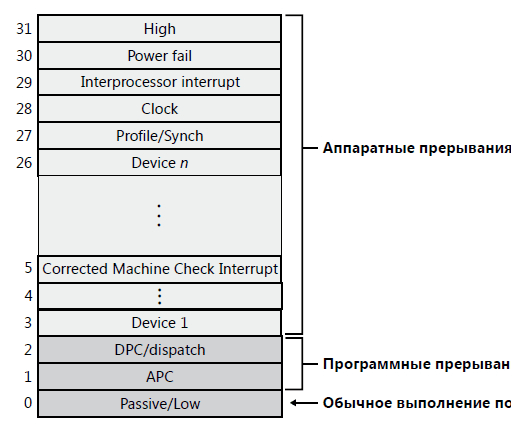
\includegraphics[scale=1]{source/arhitektura-86.png}
 		\caption*{Уровни IRQL}
 	\end{figure}
 
 	\subsection{UNIX/Linux}
 	Классическое ядро Linux было невытесняемым. Это означает, что если процесс выполняется
 	в режиме ядра, то ядро не заставит этот процесс уступить процессорное время какому-либо более приоритетному
 	процессу. Выполняющийся процесс может только добровольно освободить процессор в случае своего блокирования
 	в ожидании ресурса, иначе он может быть ветеснен при переходе в режим задачи. Такая реализация ядра позволяет решить множество проблем синхронизации, связанных с доступом нескольких процессов к одним и тем же
 	структурам данных ядра.
 	Современные ядра Linux являются полностью вытесняемыми. Это обусловлено поддержкой процессов реального времени, например видео или аудио.\par
 	
 	\textbf{Приоритеты процессов:}\par
 	Приоритет процесса в Unix задается любым целым числом в диапозоне от 0 до 127 и это число меньше,
 	тем выше приоритет. Приоритеты от 0 до 49 зарезервированы для ядра, а прикладные процессы могут обладать
 	приоритетом в диапазоне от 50 до 127.\par
 	Структура proc содержит следующие поля, относящиеся к приоритетам:
 	\begin{table}[h]
 		\begin{center}
 			\begin{tabular}{|l|l|}
 				\hline
 				p\_pri    & Текущий приоритет планирования                          \\ \hline
 				p\_usrpri & Приоритет режима задачи                                 \\ \hline
 				p\_cpu    & Результат последнего измерения использования процессора \\ \hline
 				p\_nice   & Фактор "любезности", устанавливаемый пользователем      \\ \hline
 			\end{tabular}
 		\end{center}
 	\end{table}\par
 
	 Планировщик использует p\_pri для принятия решения о том, какой процесс
	 отправить на выполнение.\par
	 Когда процесс находится в режиме задачи p\_pri и p\_usrpri идентичны.
	 Планировщик использует p\_usrpri для хранения приоритета, который будет
	 назначен процессу при возврате в режим задачи, а p\_pri — для хранения
	 временного приоритета для выполнения в режиме ядра.\par
	 Процессу, ожидающему недоступного в данный момент ресурса, система
	 определяет значение приоритет сна выбираемое ядром из диапазона 0-49 и
	 связанное с событием, вызвавшее это состояние.\par
	 Когда замороженный процесс просыпается, значение p\_pri устанавливается
	 равным приоритету сна события или ресурса, на котором он был заблокирован.
	 Системные приоритеты сна представлены в таблице ниже.
	 
	 \clearpage
	 \begin{table}[h]
	 	\begin{center}
	 		\begin{tabular}{|l|p{65pt}|p{65pt}|} 
	 			\hline
	 			{Событие} & {Приоритет 4.3BSD UNIX} & {Приоритет SCO UNIX}\\
	 			\hline
	 			{Ожидание загрузки в память страницы} & 0 & 95\\
	 			\hline
	 			{Ожидание индексного дескриптора} & 10 & 88\\
	 			\hline
	 			{Ожидание ввода--вывода} & 20 & 81 \\
	 			\hline
	 			{Ожидание буфера} & 30 & 80\\
	 			\hline
	 			{Ожидание терминального ввода} &  & 75\\
	 			\hline
	 			{Ожидание терминального вывода} &  & 74\\
	 			\hline
	 			{Ожидание завершения выполнения} &  & 73\\
	 			\hline
	 			{Ожидание события} & 40 & 66\\
	 			\hline
	 		\end{tabular}
	 	\end{center}
	 	\caption*{Системные приоритеты сна}
	 \end{table}
 	
 	Поскольку приоритеты ядра выше, такие процессы будут назначены на
 	выполнение раньше, чем другие, функционирующие в режиме задачи. Такой
 	подход позволяет системным вызовам быстро завершать работу, что является
 	желательным, так как процессы во время выполнения вызова могут занимать
 	некоторые ключевые ресурсы системы, не позволяя другим ими пользоваться.
 	Когда процесс завершил выполнение системного вызова, его приоритет
 	сбрасывается обратно в значение текущего приоритета в режиме задачи,
 	произойдет переключение контекста.\par
 	
 	Приоритет в режиме задачи зависит от "любезности" (nice) и последней измеренной величины использования процессора. Степень любезности - это число в диапозоне от 0 до 39 со значением 20 по умолчанию. Увеличение nice приводит к уменьшению приоритета. При этом суперпользователь может поднять приоритет.\par
 	
 	Системы разделения времени пытаются выделить процессорное время таким образом, чтобы конкурирующие процессы системы получили его в примерно равных количествах. Поле p\_cpu при создании процесса инициализируется нулем. На кажом тике обработчик таймера увеличивает p\_cpu на удиницу для текущего процесса до
 	максимального значения 127.\par
 	
 	Каждую секунду ядро системы вызывает процедуру руschedcpu() (запускаемую
 	через отложенный вызов), которая уменьшает значение p\_cpu каждого процесса
 	исходя из фактора «полураспада» (decay factor).\par
 	
 	По формуле:
 	\begin{equation*}
 		\text{decay} = \frac{2 * \text{load\_average}}{2 * \text{load\_average} + 1},
 	\end{equation*}
 	\noindent где load\_average - среднее количество процессов в состоянии готовности за последнюю секунду. \par
 	Процедура schedcpu() также пересчитывает приоритеты для режима задачи всех
 	процессов по формуле: 
 	\begin{equation*}
 		\text{p\_usrpri} = \text{PUSER} + (\text{p\_cpu} / 4) + (2 * \text{p\_nice}),
 	\end{equation*}
 	\noindent где PUSER - базовый приоритет в режиме задачи, равный 50.
 	
 	Если процесс в последний раз использовал большое количество процессорного времени, его p\_cpu будет увеличен, что приведет к увеличению значения p\_usrpri, и к понижению приоритета. Чем дольше процесс простаивает в очереди на выполнение, тем больше фактор полураспада уменьшает его p\_cpu, что приводит к повышению его приоритета.\par
 	В системах разделения времени фактор использования процессора обеспечивает равные и честные условия при планировании процессов. Фактор полураспада обеспечивает экспотенциально взвешенное среднее
 	значение использования процессора в течение всего периода функционирования процесса.
 	
 	\clearpage
 	\section{Заключение}
 	Операционные системы Windows и Unix/Linux - системы с разделением времени с динамическими приоритетами и вытеснением. Поэтому обработчик системного таймера выполняет похожие функции:
 	\begin{itemize}
 		\item[1)] инкремент счетчика системного времени;
 		\item[2)] декремент кванта;
 		\item[3)] добавление функций планировщика в очередь отложенных вызовов;
 		\item[4)] декремент счетчиков времени, оставшегося до выполнения отложенных вызовов;
 		\item[5)] отправка отложенных вызовов на выполнение.		
 	\end{itemize}
 	 	
	Алгоритмы планирования основаны на очередях, но работа планировщиков различна:
	планировщик в Windows вызывается самими процессами, тогда как в Unix/Linux за это отвечает ядро. 	
 
\end{document}